%%%%%%%%%%%%%%%%%%%%%%%%%%%%%%%%%%%%%%%%%%%%%%%%%%%%%%%%%%%%%%%%%%%%%%%%%%%%%%%%%%%%%%%%%%%%%
%%									section 1.	Principe Mod\`{e}le Checker Distribu\'{e}											%
%%%%%%%%%%%%%%%%%%%%%%%%%%%%%%%%%%%%%%%%%%%%%%%%%%%%%%%%%%%%%%%%%%%%%%%%%%%%%%%%%%%%%%%%%%%%%

\subsection{Principe Model Checking Distribu\'{e}}
 
Le model checking adopté est qui a été  propos\'{e} par Bouneb Zine dans sa thèse \citep{depriester2011bouneb} (voir chapitre \ref{chapmc}, section \ref{mcd}), il permet une vérification parallèles d’une formule $\varphi$  sur les fragments de la structure de Kripke distribuée. Du fait de la distribution, la vérification de $\varphi$ de certain état \emph{S} dépend de la vérité en \emph{S’} de cette formule, \emph{S’}  hébergé dans une  machine distante $M_j$. La machine $M_i$ effectue la vérification de $\varphi$ sur le fragment détenue en considérant la valeur logique de \emph{S’} indécidable  $L (\emph{S’},\varphi )=\perp$ car la formule $\varphi$ peut être vérifier en \emph{S’}. Lorsque la machine $M_j$ termine le calcul est que la formule est vérifiée en \emph{S’}, aucune notification n'est envoyée à la machine $M_i$, la machine $M_i$ considère que la formule est vérifiée en \emph{S’}, sinon la machine $M_j$ envoi à la machine $M_i$ la valeur logique de \emph{S’} qui est $L(\emph{S’}, \varphi) =false$. Dans ce cas, $M_i$ reprend le calcul de vérification avec la prise en compte de valeur envoyée afin de déterminer la logique de formule sur les états prédécesseurs. Une fois que la terminaison est détectée  la machine détenant l’état initial déduit la véracitée de la formule $\varphi$.

\begin{Exemple}
   Soit une structure de Kripke distribuée représentée sur la Figure \ref{skd1}, l'exécution du model checking de la formule \s{AG(a)} sur cette structure, ainsi les résultat obtenue sont:
   \begin{itemize}
   	\item Après une première itération l'algorithme détecte sur la machine $M_1$ que la formule n’est pas vérifiée sur l’état \s{S1}, cela nécessite l'envoyer d'une notification à la machine $M_3$ qui possède un prédécesseur direct de cet état.
   	\item Après la réception d'une notification sur la machine $M_3$ et la prise en compte de la notification sur l'état \s{S1}, l'algorithme du model checking est relancé sur la machine $M_3$. Après le processus de vérification, la valeur logique de la formule sur l’état \s{S5} est $false$ grâce à la deuxième itération. Après cela, aucune notification n'a été envoyé, sur la machine $M_3$ l'algorithme déduit alors la véracitée de la formule.
   \end{itemize}    
Les résultats observés durant le processus de vérification de la formule \s{AG(a)} sont représentés dans le Tableau \ref{statistique}, les lignes représentent les données concernant un état et les colonnes les types de données construits durant le processus de vérification. Les abréviations utilisées sont:
\begin{description}[,leftmargin=2cm,labelindent=1em]
	\item[Id   :] L'identifiant de l’état;
	\item[VL   :] La valeur logique de la formule à vérifier $(true : 1 ; false : 0 ; \perp : -1)$;
	\item [Sub :] Liste des machines sollicitant l'état;
	\item[T    :] Le type d’état (I : interne ; E : externe);
	\item[Site :] La machine distante o\`{u} l'état (Externe) réside;
	\item[I    :] La liste des itération permettant de déterminer la valeur logique de l'état.	
\end{description}
   \centering
	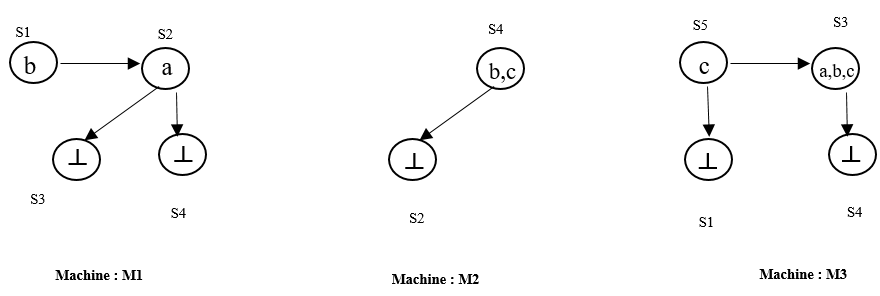
\includegraphics[height=2in]{img/skd1.png}	
	\captionof{figure}{Structure de kripke distribu\'{e}}\label{skd1}
\end{Exemple}
\begin{tableth}
	\centering
	\begin{tabular}{|c|c|c|c|c|c|c|c|c|}
		\hline
		\multicolumn{7}{|c|}{Itération 1}                                  \\ \hline
		          Machine           & Id & T & VL & I & Site &    Sub      \\ \hline
		\multirow{4}{*}{Machine M1} & S1 & I & 0  & 1 &      & \{$M_3$\}   \\ \cline{2-7}
		                            & S2 & I & -1 & 1 &      &             \\ \cline{2-7}
		                            & S3 & E & -1 & 1 &  M3  &             \\ \cline{2-7}
		                            & S4 & E & -1 & 1 &  M4  &             \\ \hline
		\multirow{2}{*}{Machine M2} & S2 & E & -1 & 1 &  M1  &             \\ \cline{2-7}
		                            & S4 & I & -1 & 1 &      &             \\ \hline
		\multirow{4}{*}{Machine M3} & S4 & E & -1 & 1 &  M2  &             \\ \cline{2-7}
		                            & S5 & I & -1 & 1 &      &             \\ \cline{2-7}
		                            & S3 & I & -1 & 1 &      &             \\ \cline{2-7}
		                            & S1 & E & -1 & 1 &  M1  &             \\ \hline
		\multicolumn{7}{|c|}{Itération 2}                                  \\ \hline
		\multirow{2}{*}{Machine M3} & S1 & E & 0  & 2 &  M1  &             \\ \cline{2-7}
		                            & S5 & I & 0  & 2 &      &             \\ \hline
	\end{tabular}
	\caption{Statistique des \'{e}tats}\label{statistique}
\end{tableth}

